% Vector figures for pages 1--2. Requires tikz, xcolor, and \ifanswers.
% The main document defines answerred. All macros take no arguments.
\usetikzlibrary{decorations.pathreplacing}
\providecommand{\FFAns}[1]{\ifanswers\textcolor{answerred}{$#1$}\else\phantom{$#1$}\fi}
\tikzset{ffbox/.style={draw,line width=.45pt,minimum width=.82cm,minimum height=.40cm,inner sep=1.5pt,font=\small},
  ffop/.style={circle,draw,line width=.45pt,minimum size=.29cm,inner sep=0pt,font=\small},
  fflink/.style={line width=.45pt},
  ffbrace/.style={decorate,decoration={brace,amplitude=3pt},line width=.4pt}}

\newcommand{\FigLines}{%
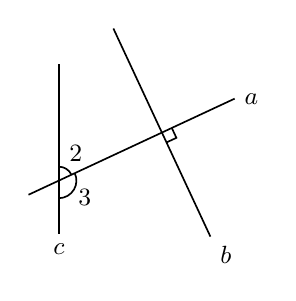
\begin{tikzpicture}[x=.77cm,y=.77cm,line width=.6pt,font=\small]
  \coordinate (O) at (2.2,1.42);
  \draw (0,.394)--(3.4,1.979) node[right]{$a$};
  \draw (1.4,3.136)--(3,-.296) node[below right]{$b$};
  \draw (.5,-.25)--(.5,2.55);
  \node[below] at (.5,-.25){$c$};
  % The square is exactly aligned with a and b (25-degree and -65-degree rays).
  \draw (2.3631,1.4961)--(2.4392,1.3330)--(2.2761,1.2569);
  \draw (.5,.6271) ++(25:.23) arc[start angle=25,end angle=90,radius=.23];
  \draw (.5,.6271) ++(-90:.29) arc[start angle=-90,end angle=25,radius=.29];
  \node at (.78,1.08){2};
  \node at (.93,.35){3};
\end{tikzpicture}}

\newcommand{\FigRoutes}{%
\begin{tikzpicture}[x=.88cm,y=.88cm,line width=.55pt,font=\small]
  \draw (0,2.10)--(4,2.10) (0,2.65)--(4,2.65);
  \node at (2,2.375){五一大街};
  \coordinate (H) at (2,0);
  \draw (H)..controls (1.40,.10) and (1.65,.55)..(1.05,.65)
    ..controls (.18,.8) and (.50,1.45)..(.15,2.10);
  \draw (H)--(2,2.10);
  \draw (H)--(2.75,2.10);
  \draw (H)..controls (3.65,.65) and (3.9,.85)..(3.85,2.10);
  \draw (2,1.91)--(2.19,1.91)--(2.19,2.10);
  \fill (H) circle[radius=1.5pt];
  \node[below] at (H){李芳家};
  \node at (.96,.42){$A$};
  \node[left] at (1.98,1.13){$B$};
  \node[right] at (2.46,1.07){$C$};
  \node[right] at (3.67,1.03){$D$};
\end{tikzpicture}}

\newcommand{\FigReceipt}{%
\begin{tikzpicture}[x=1cm,y=1cm,font=\small]
  \draw[line width=.55pt] (0,0) rectangle (3.65,1.72);
  \node[anchor=west] at (.15,1.42){单价：58元/件};
  \node[anchor=west] at (.15,1.04){数量：};
  \ifanswers
    \node[anchor=west,text=answerred] at (1.22,1.04){17};
  \else
    \fill[gray!35] (1.23,.89) rectangle (1.80,1.19);
  \fi
  \node[anchor=west] at (1.86,1.04){件};
  \node[anchor=west] at (.15,.66){付款金额：1000元};
  \node[anchor=west] at (.15,.28){找零：14元};
\end{tikzpicture}}

\newcommand{\FigTreeA}{%
\begin{tikzpicture}[x=.82cm,y=.71cm]
  \node[ffbox] (a) at (2.4,3.2){\FFAns{14}};
  \node[ffop] at (3.15,3.2){\FFAns{-}};
  \node[ffbox] (b) at (3.9,3.2){\FFAns{12}};
  \node[ffbox] (c) at (3.15,2.2){\FFAns{2}};
  \node[ffbox] (d) at (1.65,2.2){\FFAns{15}};
  \node[ffop] at (2.4,2.2){\FFAns{\times}};
  \node[ffbox] (e) at (2.4,1.2){\FFAns{30}};
  \node[ffbox] (f) at (.9,1.2){\FFAns{990}};
  \node[ffop] at (1.65,1.2){\FFAns{-}};
  \node[ffbox] (g) at (1.65,.2){\FFAns{960}};
  \draw[fflink] (a.south)--(c.north) (b.south)--(c.north)
    (c.south)--(e.north) (d.south)--(e.north)
    (e.south)--(g.north) (f.south)--(g.north);
\end{tikzpicture}}

\newcommand{\FigMultiplication}{%
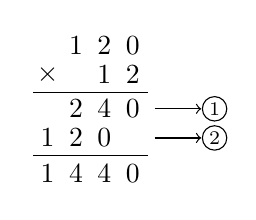
\begin{tikzpicture}[x=1cm,y=1cm,font=\normalsize]
  % Four fixed columns guarantee correct positional alignment.
  \node at (.36,1.82){$1$}; \node at (.72,1.82){$2$}; \node at (1.08,1.82){$0$};
  \node at (0,1.45){$\times$}; \node at (.72,1.45){$1$}; \node at (1.08,1.45){$2$};
  \draw[line width=.55pt] (-.18,1.23)--(1.28,1.23);
  \node at (.36,1.02){$2$}; \node at (.72,1.02){$4$}; \node at (1.08,1.02){$0$};
  \node at (0,.65){$1$}; \node at (.36,.65){$2$}; \node at (.72,.65){$0$};
  \draw[line width=.55pt] (-.18,.43)--(1.28,.43);
  \node at (0,.20){$1$}; \node at (.36,.20){$4$}; \node at (.72,.20){$4$}; \node at (1.08,.20){$0$};
  \draw[->,line width=.45pt] (1.36,1.02)--(1.95,1.02);
  \node[circle,draw,inner sep=1pt,font=\scriptsize] at (2.12,1.02){1};
  \draw[->,line width=.45pt] (1.36,.65)--(1.95,.65);
  \node[circle,draw,inner sep=1pt,font=\scriptsize] at (2.12,.65){2};
\end{tikzpicture}}

\newcommand{\FigChainOne}{%
\begin{tikzpicture}[x=.84cm,y=.70cm]
  \node[ffbox] (a) at (1.8,3.2){$52$};
  \node at (2.6,3.2){$+$};
  \node[ffbox] (b) at (3.4,3.2){$29$};
  \node[ffbox] (c) at (2.6,2.2){\FFAns{81}};
  \node[ffbox] (d) at (1,2.2){$26$};
  \node at (1.8,2.2){$\times$};
  \node[ffbox] (e) at (1.8,1.2){\FFAns{2106}};
  \node at (2.6,1.2){$-$};
  \node[ffbox] (f) at (3.4,1.2){$128$};
  \node[ffbox] (g) at (2.6,.2){\FFAns{1978}};
  \draw[fflink] (a.south)--(c.north) (b.south)--(c.north)
    (c.south)--(e.north) (d.south)--(e.north)
    (e.south)--(g.north) (f.south)--(g.north);
\end{tikzpicture}}

\newcommand{\FigChainTwo}{%
\begin{tikzpicture}[x=.84cm,y=.70cm]
  \node[ffbox] (a) at (1,3.2){$212$};
  \node at (1.8,3.2){$+$};
  \node[ffbox] (b) at (2.6,3.2){$460$};
  \node[ffbox] (c) at (1.8,2.2){\FFAns{672}};
  \node at (2.6,2.2){$\div$};
  \node[ffbox] (d) at (3.4,2.2){$24$};
  \node[ffbox] (e) at (2.6,1.2){\FFAns{28}};
  \node[ffbox] (f) at (1,1.2){$20$};
  \node at (1.8,1.2){$\times$};
  \node[ffbox] (g) at (1.8,.2){\FFAns{560}};
  \draw[fflink] (a.south)--(c.north) (b.south)--(c.north)
    (c.south)--(e.north) (d.south)--(e.north)
    (e.south)--(g.north) (f.south)--(g.north);
\end{tikzpicture}}

\newcommand{\FigRelations}{%
\begin{tikzpicture}[x=1cm,y=1cm,font=\small,line width=.5pt]
  \foreach \x/\lab/\ffouter/\ffinner in {0/A/相交/互相垂直,3.9/B/相交/互相平行,7.8/C/互相平行/互相垂直}{
    \begin{scope}[xshift=\x cm]
      \node at (.05,.94){\lab.};
      \draw (1.85,.93) ellipse[x radius=1.50,y radius=.70];
      \node at (1.85,1.28){\ffouter};
      \draw (1.85,.70) ellipse[x radius=1.02,y radius=.27];
      \node at (1.85,.70){\ffinner};
    \end{scope}
  }
\end{tikzpicture}}

\newcommand{\FigBars}{%
\begin{tikzpicture}[x=1cm,y=1cm,font=\footnotesize,line width=.5pt]
  % A: known whole and one known part.
  \begin{scope}
    \node at (0,.71){A.};
    \draw (.35,.61) rectangle (3.00,.81);
    \draw (1.02,.61)--(1.02,.81);
    \draw[ffbrace] (.35,.94)--(1.02,.94) node[midway,above=3pt]{16元};
    \draw[ffbrace] (1.02,.94)--(3.00,.94) node[midway,above=3pt]{?元};
    \draw[ffbrace] (3.00,.45)--(.35,.45) node[midway,below=3pt]{50元};
  \end{scope}
  % B: sum of three different prices.
  \begin{scope}[xshift=3.8cm]
    \node at (0,.71){B.};
    \draw (.35,.61) rectangle (3.00,.81);
    \draw (1.00,.61)--(1.00,.81) (1.80,.61)--(1.80,.81);
    \draw[ffbrace] (.35,.94)--(1.00,.94) node[midway,above=3pt,xshift=-2pt]{10元};
    \draw[ffbrace] (1.00,.94)--(1.80,.94) node[midway,above=3pt,xshift=2pt]{14元};
    \draw[ffbrace] (1.80,.94)--(3.00,.94) node[midway,above=3pt]{26元};
    \draw[ffbrace] (3.00,.45)--(.35,.45) node[midway,below=3pt]{?元};
  \end{scope}
  % C: 48 yuan plus 16 yuan; the common part is three equal units.
  \begin{scope}[xshift=7.6cm]
    \node at (0,.71){C.};
    \draw (.35,1.00) rectangle (2.33,1.20);
    \draw (1.01,1.00)--(1.01,1.20) (1.67,1.00)--(1.67,1.20);
    \draw[ffbrace] (.35,1.33)--(2.33,1.33) node[midway,above=3pt]{48元};
    \draw (.35,.45) rectangle (2.99,.65);
    \draw (1.01,.45)--(1.01,.65) (1.67,.45)--(1.67,.65) (2.33,.45)--(2.33,1.20);
    \draw[ffbrace] (2.33,.78)--(2.99,.78) node[midway,above=3pt]{16元};
    \draw[ffbrace] (2.99,.29)--(.35,.29) node[midway,below=3pt]{?元};
  \end{scope}
  % D: five equal portions. Unit price is 130 yuan.
  \begin{scope}[xshift=11.4cm]
    \node at (0,.71){D.};
    \draw (.35,.61) rectangle (3.00,.81);
    \foreach \x in {.88,1.41,1.94,2.47}{\draw (\x,.61)--(\x,.81);}
    \draw[ffbrace] (.35,.94)--(.88,.94) node[midway,above=3pt]{130元};
    \draw[ffbrace] (3.00,.45)--(.35,.45) node[midway,below=3pt]{?元};
  \end{scope}
\end{tikzpicture}}
